\documentclass[a4paper,11pt]{article}
\usepackage[margin=2cm]{geometry}

\usepackage[nodayofweek]{datetime}
\usepackage{cite}
\usepackage{graphicx}
\longdate

\usepackage{hyperref}
\usepackage{fancyhdr}
\pagestyle{fancyplain}
\fancyhf{}
\lhead{\fancyplain{}{M.Sc.\ Group Project Report}}
\rhead{\fancyplain{}{\today}}
\cfoot{\fancyplain{}{\thepage}}


\title{Implementation of attentional bistability of the dragonfly visual neurons in an intelligent biomimetic agent\\\Large{--- Final Report ---}}
\author{Juan Carlos Farah, Panagiotis Almpouras, Ioannis Kasidakis, Erik Grabljevec, Christos Kaplanis\\
       \{jcf214, pa512, ik311, eg1114, ck2714\}@doc.ic.ac.uk\\ \\
       \small{Supervisors: Professor Murray Shanahan, Zafeirios Fountas, Pedro Mediano}\\
       \small{Course: CO530/533, Imperial College London}
}

\begin{document}
\maketitle

\section{Design}

After in depth research and careful consideration we managed to identify the necessary components to replicate a coherent visual system.
There are six main modules this project comprises of. This section provides the design overview of each as well as how they are interconnected to work as a single system.

\begin{enumerate}
\item{Target Animation:} Provides the visual input that is then translated to a spike train. For such a generic task, a lot of programming languages provide strong supporting tools. To enhance the uniformity of the project as a whole we decided to use Python.\cite{python}
\item{Elementary Small Target Motion Detector (ESTMD):} The ESTMD neuron has the function of identifying and isolating small moving targets, even against a cluttered, moving background (WIEDERMAN 2008). Our ESTMD component models that behaviour essentially preprocessing the visual input before it reaches the CSTMD.
\item{Centrifugal Small Target Motion Detector (CSTMD):} The CSTMD neuron is a higher order visual neuron in the brain of the dragonfly. This neuron reacts to the presentation of multiple visual stimuli by firing as if only one of the stimuli was present \cite{w13}. By modelling that behaviour a target selection mechanism can be implemented.
\item{Pattern Recognition:} By exploiting the effect of the Spike Timing Dependent Plasticity (STDP) a powerful pattern recognition mechanism was built\cite{stdp1}\cite{stdp2}. This mechanism enables the identification of the direction of movement of the animated target.
\item{Action Selection:} Using reward modulated re-enforcement learning along with the output of the pattern recognition neurons this module is responsible for the movement of the dragonfly towards the animated target.It includes an animation component for the visualisation of the outcome.
\item{Web Client:} Although this is not a module that is actively implicated in the neural processes that are being modelled in this project, it is a very powerful tool that drastically enhances the functionality of the system. The web client is connected to every component providing a user friendly interface that allows not only the independent use of each of the components but also to run simulations using the system as a whole. The web client provides the user with an output that is crucial in understanding the performance of the system. It allows for flexibility as the users may set their own parameters and run, save and load simulations.
\end{enumerate}

The following figure provides a graphical representation of the system as whole. The animated target acts as input to the ESTMD neuron which identifies and isolates the small targets (if any) by processing each frame of the animation. The output of the ESTMD is yet another animation but this time the only things visible are the small targets. This new animation acts as input to the CSTMD neuron. In the presence of multiple targets, a well behaved CSTMD neuron should select one and translate only that target's movement into a spike train which will be processed by the pattern recognition neurons. In this spike train a pattern exists that encodes information about the direction of the selected target. The pattern recognition neuron trained to identify that particular pattern will fire - upon recognition of the pattern - while inhibiting the rest of the pattern recognition neurons. The action selection mechanism then has to translate the output of the pattern recognition (i.e. the spike from a neuron) to an action that ideally will bring the dragonfly closer to its prey.
The web client "oversees" the whole process ensuring that the components are well connected and provides the user with key metrics regarding the performance of the system (or an individual module) for a particular simulation. The database stores animations, simulations and their respective results enabling their reloading if a future reference is desired.

\begin{figure}[hb]
\centering
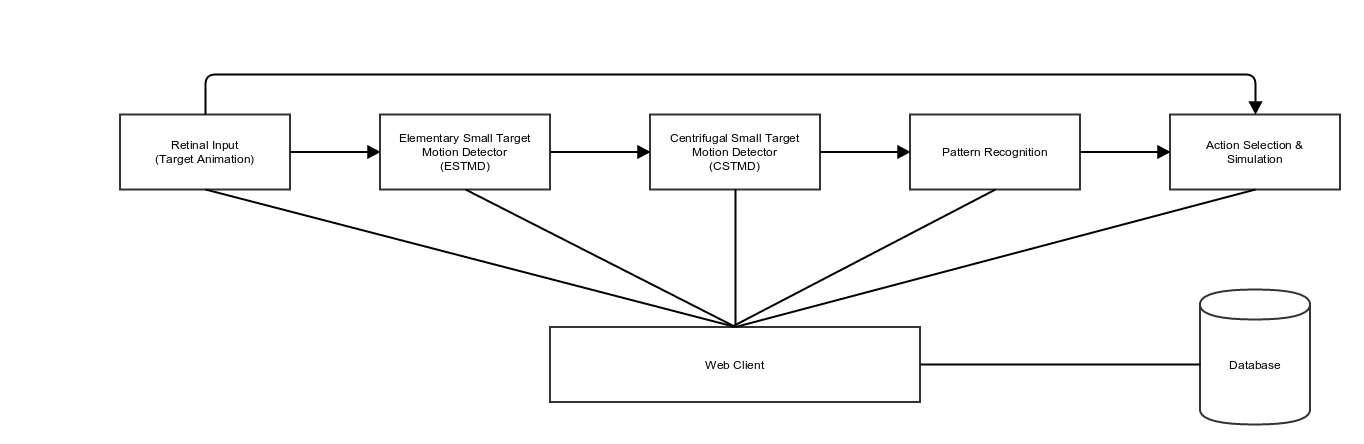
\includegraphics[scale = 0.3]{designblockdiagram}
\caption{Project Structure Diagram.}
\end{figure}


The programming language used throughout the project was Python \cite{python}. Python includes libraries that allow for efficient matrix manipulations that were key in most of the modules. Matlab was an alternative we initially considered \cite{matlab}. Although Matlab is very powerful and user friendly for some particular tasks, it does not allow for the flexibility that Python does. For that reason Matlab was disregarded as an option.
The database we used was MongoDB for ..............




\end{document}

